\documentclass{sig-alternate-05-2015}
\usepackage{graphicx,color}
\usepackage{subcaption}
\usepackage[utf8]{inputenc}
\usepackage{rotating}
\usepackage{pdflscape}
\usepackage[table,xcdraw]{xcolor}
\begin{document}

% Copyright
%\setcopyright{acmcopyright}
%\setcopyright{acmlicensed}
%\setcopyright{rightsretained}
%\setcopyright{usgov}
%\setcopyright{usgovmixed}
%\setcopyright{cagov}
%\setcopyright{cagovmixed}

\title{LaTeX Tables and Figures MegaDump}
%\title{Needs a better, witty title}


\numberofauthors{1} %  in this sample file, there are a *total*
% of EIGHT authors. SIX appear on the 'first-page' (for formatting
% reasons) and the remaining two appear in the \additionalauthors section.
%

\author{
% 1st. author
\alignauthor
Harsh Thakkar\\
       \affaddr{Enterprise Information Systems Lab}\\
       \affaddr{University of Bonn}\\
       \affaddr{Bonn, Germany}\\
       \email{hthakkar@uni-bonn.de}
% 2nd. author
}

%\additionalauthors{Additional authors: John Smith (The Th{\o}rv{\"a}ld Group,
%email: {\texttt{jsmith@affiliation.org}}) and Julius P.~Kumquat
%(The Kumquat Consortium, email: {\texttt{jpkumquat@consortium.net}}).}

%\date{30 July 1999}


\maketitle
\begin{abstract}
The abstract goes here \dots
\end{abstract}


%
% The code below should be generated by the tool at
% http://dl.acm.org/ccs.cfm
% Please copy and paste the code instead of the example below. 
%
%\begin{CCSXML}
%\end{CCSXML}



%
% End generated code
%

%
%  Use this command to print the description
%
\printccsdesc

% We no longer use \terms command
%\terms{Theory}

\keywords{ACM proceedings; \LaTeX; text tagging}
%===================================================
%-------------all figures---------------------------
%===================================================

\section{Figures a-la-carte}\label{figs}

\textbf{One.} Figures~\ref{fig:plot1} and \ref{fig:plot2} are for a one-column article format. It layouts both the figures side by side in it. When I tried to use it in this two-coulmn format, what happens you can see yourself.
\begin{figure}
    \centering
    \begin{subfigure}{0.4\textwidth}
        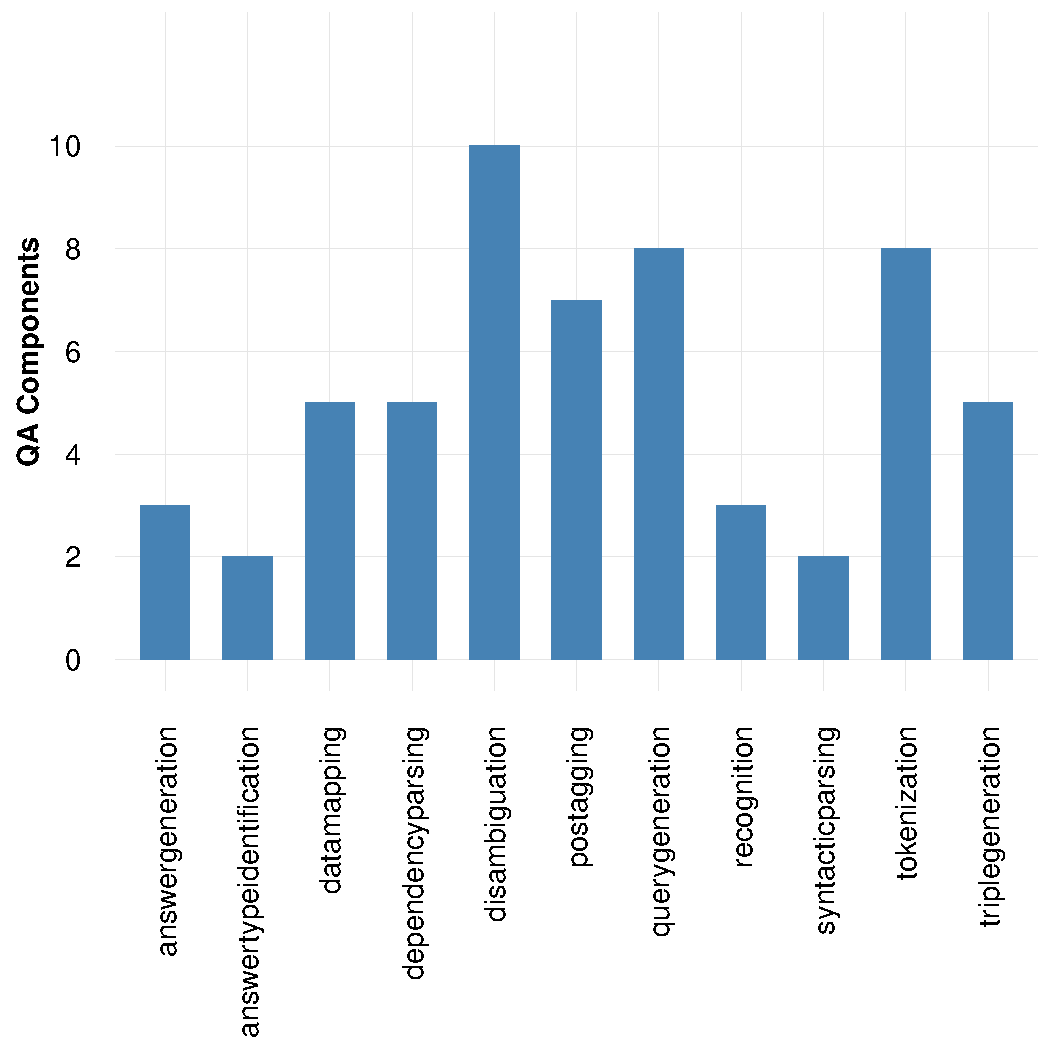
\includegraphics[width=0.5\textwidth]{figures/plot1}
        \subcaption{QA Components per QA Task}
        \label{fig:plot1}
    \end{subfigure}
    \begin{subfigure}{0.4\textwidth}
        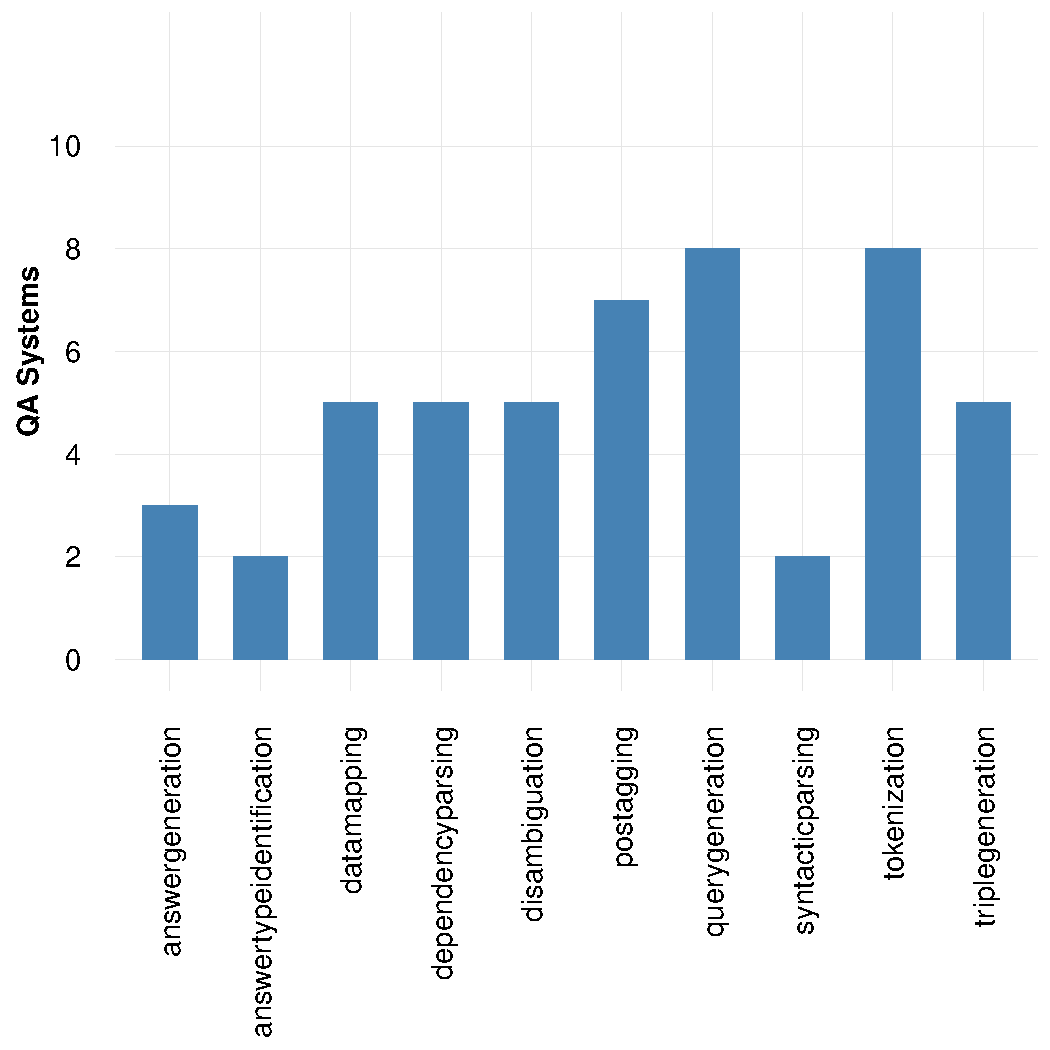
\includegraphics[width=0.5\textwidth]{figures/plot2}
        \subcaption{QA Systems per QA Task}
        \label{fig:plot2}
    \end{subfigure}
    \caption{{\bf Frequencies of QA components and Systems per QA Task}. Disambiguation, Tokenization, and Query Generation are the most popular tasks.}
    \label{fig:qaestro-components}
\end{figure}


\textbf{Two.} The second figure~\ref{plot2}, is an example of a figure for two column format. We define the width to be that of \texttt{linewidth}, unlike example 1 where we scale the actual figure ot its 10\% size.
\begin{figure}
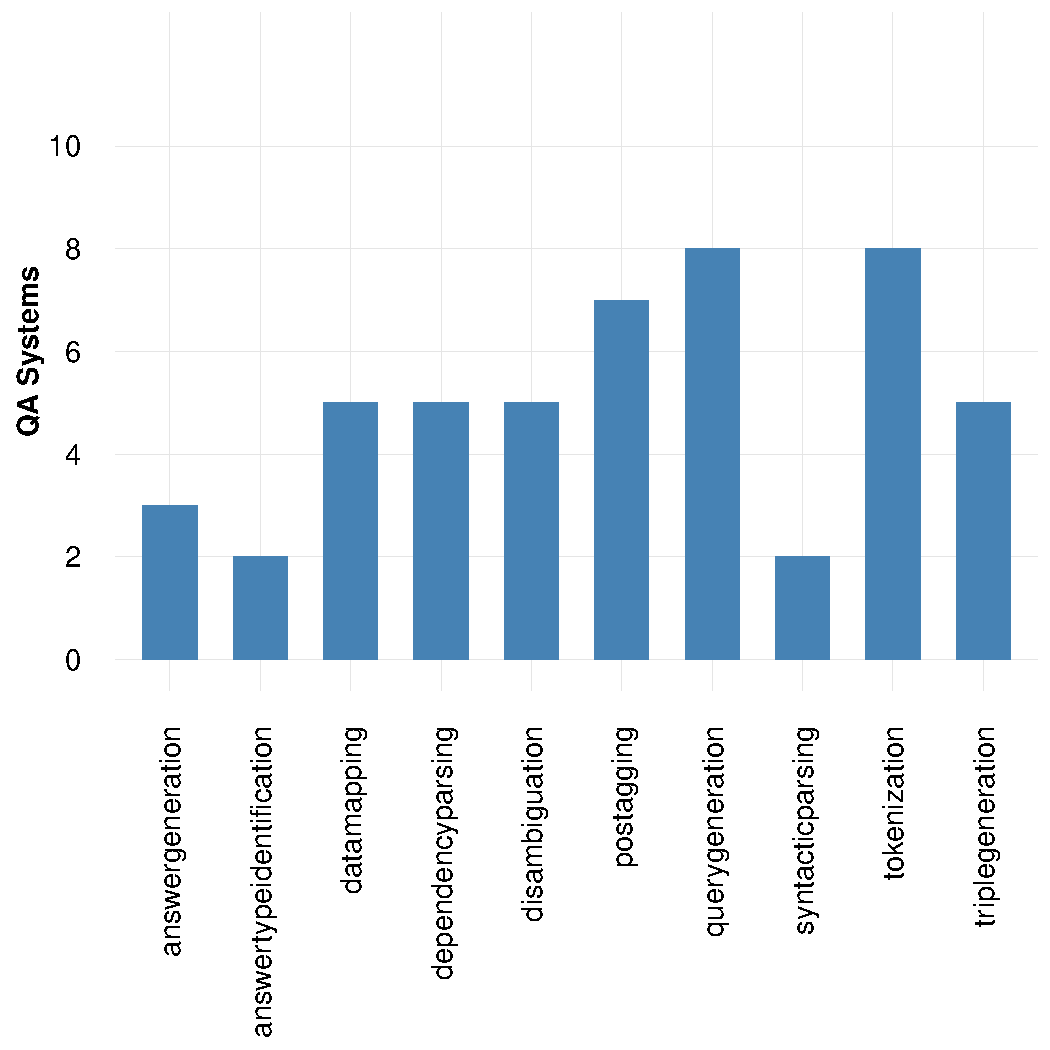
\includegraphics[width=0.45\textwidth]{figures/plot2}
\caption{The star category distribution of the 1st quarter of reviews dataset}
\label{plot2}
\end{figure}


\textbf{Three.} A full page \texttt{sideways} figure (ref. Figure~\ref{fig:metadataAccessibility}).
\begin{sidewaysfigure*}
 \centering
 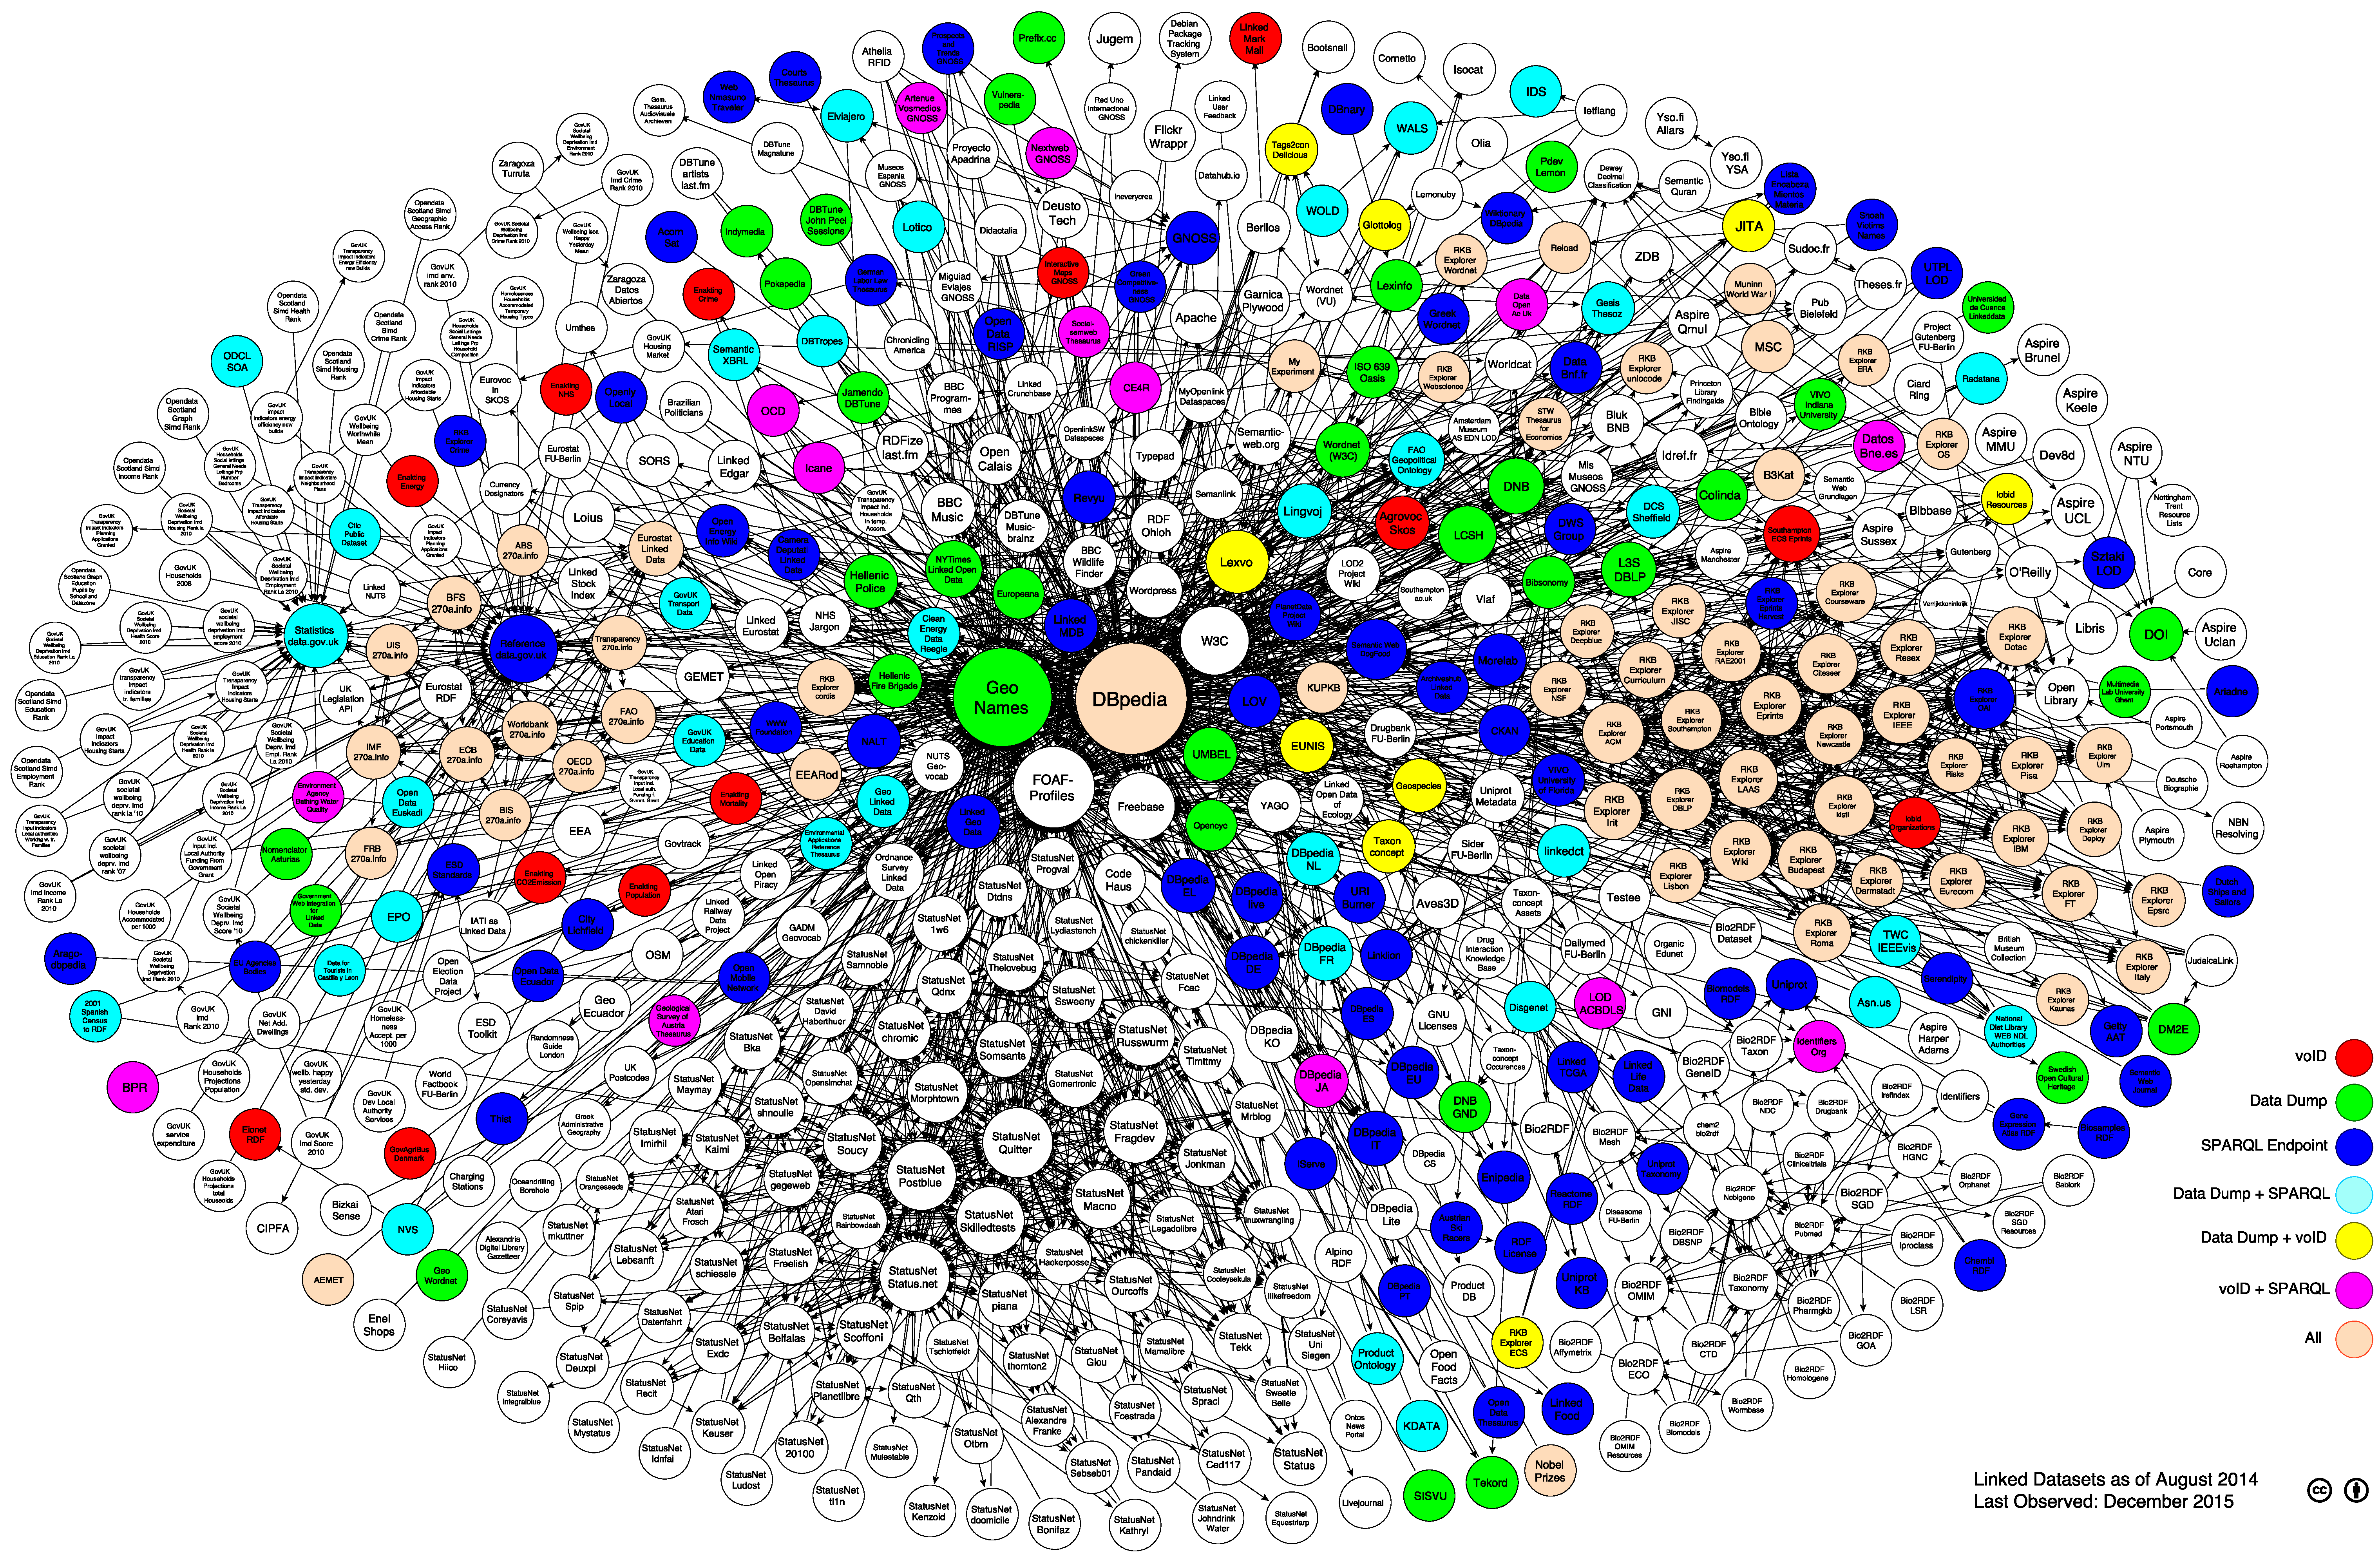
\includegraphics[width=\textwidth]{figures/lod-cloud-metadata-accessibility.pdf}
  \caption{Coloring the LOD Cloud Datasets with various Access Methods (Data Dump, voID, SPARQL Endpoint, or a combination)}
  \label{fig:metadataAccessibility}
\end{sidewaysfigure*}

%===================================================
%--------------all tables -------------------------
%===================================================

\section{Tables a-la-carte}\label{tabs}

You can also use http://www.tablesgenerator.com/ for the ease of human life.

\textbf{Second} example of a simple table, with the size that fits in one column of the two, and in place of the text (ref.~\ref{tab2}):
\begin{table}[htbp]
\centering
    \caption{Results of Pearson Correlation Test}
    \label{tab2}
\begin{tabular}{|l|l|l|}
    \hline
    \textbf{R value} & \textbf{P value} & \textbf{Stderr} \\ \hline
    0.3219           & 0.0              & 0.0040          \\ \hline
    \end{tabular}
\end{table}

\textbf{Third.} A table with new features:

\begin{table}[htbp]
\caption{Naive Inverted Index. TODO: Values > 1} % If we support frequencies greater than 1, then this should be in the example table.
\label{tab:Resource-based-Inverted-Index}
\centering
\scriptsize
\begin{tabular}{llllllllllll}
\textbf{row} & \textbf{Term}  & \multicolumn{9}{c}{\textbf{Resources}} \\
\cline{3-11}
& & \textbf{r1} & \textbf{r2} & \textbf{r3}  & \textbf{t1} & \textbf{t2} & \textbf{p1} & \textbf{p2}& \textbf{p3}& \textbf{p4}\\
1 & garry    & 1          & 0         & 0 &  0   &   0 &   0 &   0 &   0 &   0\\
2   &   marshall & 1          & 0         & 0 &  0   &   0 &   0 &   0 &   0 &   0\\
3   &   pretty & 0          & 0         & 1 &  0   &   0 &   0 &   0 &   0 &   0\\
4   &   woman & 0         & 0        & 1 &  0   &   0 &   0 &   0 &   0 &   0\\
5   &   dear & 0          & 1         & 0 &  0   &   0 &   0 &   0 &   0 &   0\\
6   &   god  & 0          & 1         & 0 &  0   &   0 &   0 &   0 &   0 &   0\\
7   &   actor & 1          & 0         & 0 &  0   &   0 &   0 &   0 &   0 &   0\\
8   &   writer & 1          & 0         & 0 &  0   &   0 &   0 &   0 &   0 &   0\\
9   &   producer & 1          & 0         & 0 &  0   &   0 &   0 &   0 &   0 &   0\\
10   &   direct & 1          & 0         & 0 &  0   &   0 &   0 &   0 &   1 &   0\\
11   &   person & 0          & 0         & 0 &  1   &   0 &   0 &   0 &   0 &   0\\
12  &   movie & 0          & 0         & 0 &  0   &   1 &   0 &   0 &   0 &   0\\
13   &   label    & 0          & 0         & 0 &  0   &   0 &   1 &   0 &   0 &   0\\
14   &   type     & 0          & 0         & 0 &  0   &   0 &   0 &   1 &   0 &   0\\
15   &   occupation & 0          & 0         & 0 &  0   &   0 &   0 &   0 &   0 &   1\\
\end{tabular}
\end{table}


\textbf{First} example of a for one column format when used in a two column environment, this is what happens (ref. Table~\ref{comp_table_indexing}). It uses a \texttt{resizebox} command to contain the entire table with the text preserved within the text width, otherwise it would jus overflow the width and the table will appear as cut. One can also use it for a full page table in a two-column environment.

\begin{table}
\centering
\resizebox{\textwidth}{!}{%
\begin{tabular}{|l|l|l|}
\hline
\textbf{System} & \textbf{Data structure used} & \textbf{Platform used for indexing} \\ \hline
\textbf{SWSE/YARS2} & Sparse, Inverted Indices for RDF quads & Lucene \\ \hline
\textbf{SINDICE} & Inverted Index and On-disk persistent storage & Solr \\ \hline
\textbf{SINA} & Bitmap index on RDF quads (toal 5 indices are maintained: 2 full rdf quad indices, 3 partial rdf quad indices) & OpenLink Virtuoso \\ \hline
\textbf{HAWK} & *N/A & *N/A \\ \hline
\textbf{TBSL} & Inverted Index & Solr \\ \hline
\textbf{EYPHRA} & Inverted index & Lemur-Indri \\ \hline
\hline
\end{tabular}
}
\caption{A table comparing the indexing platforms and data structures used by a variety of question answering systems.}
\label{comp_table_indexing}
\end{table}


Full page table example (ref. Table~\ref{tbl:metadata_machine_readable_licenses}).
\begin{table*}
\centering
\resizebox{\textwidth}{!}{%
\begin{tabular}{|l|l|l|c|c|}
\hline
\multicolumn{1}{|c|}{\textbf{License Used}} & \multicolumn{1}{c|}{\textbf{Type of License}} & \multicolumn{1}{c|}{\textbf{URL Used}} & \textbf{\begin{tabular}[c]{@{}c@{}}Semantic\\ Resource\end{tabular}} & \textbf{Frequency} \\ \hline
\begin{tabular}[c]{@{}l@{}}Creative Commons \\ Attribution License\end{tabular}                          & Requires Attribution  & http://www.opendefinition.org/licenses/cc-by & \ding{55} & 93 (+2)            \\ \hline
\begin{tabular}[c]{@{}l@{}}Creative Commons \\ Attribution Share-Alike \\ License\end{tabular} & Requires Attribution and Share Alike & http://www.opendefinition.org/licenses/cc-by-sa & \ding{55} & 47 (+1)            \\ \hline
\begin{tabular}[c]{@{}l@{}}Creative Commons Attribution \\ Non-Commercial \\ V2.0 License\end{tabular}   & \begin{tabular}[c]{@{}l@{}}Requires Attribution but dataset cannot be used \\ for commercial purposes. This license is a \\ non-conformant license for open data.\end{tabular} & http://creativecommons.org/licenses/by-nc/2.0/ & \ding{51} & 31 (+1)            \\ \hline
\begin{tabular}[c]{@{}l@{}}Creative Commons \\ CC Zero License\end{tabular} & Public domain waiving all rights on the data & http://www.opendefinition.org/licenses/cc-zero          & \ding{55} & 30 (+1)            \\ \hline
Open Database License & Requires Attribution and Share Alike & http://www.opendefinition.org/licenses/odc-odbl & \ding{55} & 9                  \\ \hline
\begin{tabular}[c]{@{}l@{}}Open Government \\ License for Public \\ Sector Information\end{tabular} & \begin{tabular}[c]{@{}l@{}}Requires Attribution. License can only be used \\ by third parties licensed by the UK Government\end{tabular}  &  http://reference.data.gov.uk/id/open-government-licence & \ding{51} & 6                  \\ \hline
\begin{tabular}[c]{@{}l@{}}Open Data Commons \\ Public Domain \\ Dedication and Licence\end{tabular}     & Public domain waiving all rights on the data & http://www.opendefinition.org/licenses/odc-pddl & \ding{55} & 5 (+1)             \\ \hline
\begin{tabular}[c]{@{}l@{}}Open Data Commons\\ Attribution License\end{tabular}                          & Requires Attribution & http://www.opendefinition.org/licenses/odc-by & \ding{55} & 5                  \\ \hline
\begin{tabular}[c]{@{}l@{}}GNU Free \\ Documentation \\ License\end{tabular} & Share Alike &  http://www.opendefinition.org/licenses/gfdl & \ding{55} & 4                  \\ \hline
\begin{tabular}[c]{@{}l@{}}Creative Commons \\ Attribution-NonCommercial-\\ ShareAlike V3.0\end{tabular} & \begin{tabular}[c]{@{}l@{}}Requires Attribution and Share Alike but \\ dataset cannot be used for commercial purposes.\end{tabular} & \multicolumn{1}{c|}{-}  & - & (+2) \\ \hline
OS Open Data License & Requires Attribution and Share Alike & \multicolumn{1}{c|}{-} & - & (+2)               \\ \hline
Eurostat Policy & Requires Attribution &  \multicolumn{1}{c|}{-} & - & (+1)               \\ \hline
Project Gutenberg License  & Restricts Commercial Use    & \multicolumn{1}{c|}{-}   & - & (+1)               \\ \hline
\begin{tabular}[c]{@{}l@{}}Creative Commons\\ Attribution-NoDerivs \\ License\end{tabular}               & \begin{tabular}[c]{@{}l@{}}Does not allow work to be re-used \\ in derivative works\end{tabular}   & \multicolumn{1}{c|}{-}  & -  & (+1)  \\ \hline
\end{tabular}
}
\label{tbl:metadata_machine_readable_licenses}
\caption{List of licenses used in the metadata, extracted by machine readable properties and from human readable descriptions (values in brackets).}
\end{table*}


\textbf{Side table example.} one column table for a two coulmn format with multicolumn command (ref. Table~\ref{tbl:tb5V1}):
\begin{table}[]
\begin{tabular}{lc}
\hline
\multicolumn{1}{l|}{\textbf{Dataset}}          & \textbf{V1(D)} \\ \hline
\multicolumn{1}{l|}{zbw.eu/stw}                  & 4               \\
\multicolumn{1}{l|}{linkedmarkmail.wikier.org}   & 3               \\
\multicolumn{1}{l|}{nhs.psi.enakting.org}        & 3               \\
\multicolumn{1}{l|}{population.psi.enakting.org} & 3               \\
\multicolumn{1}{l|}{crime.psi.enakting.org}      & 3               \\
\multicolumn{2}{c}{\dots}                                            \\
\multicolumn{1}{l|}{vocab.nerc.ac.uk}            & 0               \\
\multicolumn{1}{l|}{wals.info}                   & 0               \\
\multicolumn{1}{l|}{www.productontology.org}     & 0               \\
\multicolumn{1}{l|}{bfs.270a.info}               & 0               \\
\multicolumn{1}{l|}{cordis.rkbexplorer.com}      & 0               \\ \hline
\end{tabular}
\caption{Top and Bottom 5 Ranked Datasets for the Different Serialisation\\\hspace{\textwidth} Formats Metric.}
\label{tbl:tb5V1}	
\end{table}


\textbf{Yet another} multicolumn full page table, demostrating how to summarise a huge table by adding dots in the middle of it (ref. Table~\ref{tbl:tb5ContextualOverall}).
\begin{table*}[]
\centering
\begin{tabular}{lcccccc}
\hline
\multicolumn{1}{l|}{\textbf{Dataset}}                         & \multicolumn{1}{c|}{\textbf{$v(C,1.0)$}} & \multicolumn{1}{c|}{\textbf{P1}} & \multicolumn{1}{c|}{\textbf{P2}} & \multicolumn{1}{c|}{\textbf{U1}} & \multicolumn{1}{c|}{\textbf{U3}} & \textbf{U5} \\ \hline
\multicolumn{1}{l|}{http://bfs.270a.info/}                    & \multicolumn{1}{c|}{60.35\%}              & \multicolumn{1}{c|}{100\%}       & \multicolumn{1}{c|}{74.80\%}        & \multicolumn{1}{c|}{99.91\%}       & \multicolumn{1}{c|}{0\%}         & 0\%         \\
\multicolumn{1}{l|}{http://lod.geospecies.org}                & \multicolumn{1}{c|}{60.29\%}              & \multicolumn{1}{c|}{99.98\%}       & \multicolumn{1}{c|}{0\%}         & \multicolumn{1}{c|}{47.82\%}        & \multicolumn{1}{c|}{100\%}       & 64\%        \\
\multicolumn{1}{l|}{http://statistics.data.gov.uk/}           & \multicolumn{1}{c|}{43.05\%}              & \multicolumn{1}{c|}{0\%}         & \multicolumn{1}{c|}{0\%}         & \multicolumn{1}{c|}{98.33\%}        & \multicolumn{1}{c|}{100\%}       & 60\%        \\
\multicolumn{1}{l|}{http://www.kupkb.org/}                    & \multicolumn{1}{c|}{41.66\%}              & \multicolumn{1}{c|}{100\%}       & \multicolumn{1}{c|}{0\%}         & \multicolumn{1}{c|}{100\%}       & \multicolumn{1}{c|}{0\%}         & 0\%         \\
\multicolumn{1}{l|}{http://rod.eionet.europa.eu/}             & \multicolumn{1}{c|}{41.66\%}              & \multicolumn{1}{c|}{100\%}       & \multicolumn{1}{c|}{0\%}         & \multicolumn{1}{c|}{100\%}       & \multicolumn{1}{c|}{0\%}         & 0\%         \\
\multicolumn{7}{c}{\dots}                                                                                                                                                                                                                                            \\
\multicolumn{1}{l|}{http://curriculum.rkbexplorer.com}                      & \multicolumn{1}{c|}{0\%}               & \multicolumn{1}{c|}{0\%}         & \multicolumn{1}{c|}{0\%}         & \multicolumn{1}{c|}{0\%}         & \multicolumn{1}{c|}{0\%}         & 0\%         \\
\multicolumn{1}{l|}{http://extbi.lab.aau.dk/resource/Dataset} & \multicolumn{1}{c|}{0\%}               & \multicolumn{1}{c|}{0\%}         & \multicolumn{1}{c|}{0\%}         & \multicolumn{1}{c|}{0\%}         & \multicolumn{1}{c|}{0\%}         & 0\%         \\
\multicolumn{1}{l|}{http://data.dcs.shef.ac.uk/}              & \multicolumn{1}{c|}{0\%}               & \multicolumn{1}{c|}{0\%}         & \multicolumn{1}{c|}{0\%}         & \multicolumn{1}{c|}{0\%}         & \multicolumn{1}{c|}{0\%}         & 0\%         \\
\multicolumn{1}{l|}{http://prefix.cc/}                        & \multicolumn{1}{c|}{0\%}               & \multicolumn{1}{c|}{0\%}         & \multicolumn{1}{c|}{0\%}         & \multicolumn{1}{c|}{0\%}         & \multicolumn{1}{c|}{0\%}         & 0\%         \\
\multicolumn{1}{l|}{http://id.ndl.go.jp/auth/ndla}            & \multicolumn{1}{c|}{0\%}               & \multicolumn{1}{c|}{0\%}         & \multicolumn{1}{c|}{0\%}         & \multicolumn{1}{c|}{0\%}         & \multicolumn{1}{c|}{0\%}         & 0\%    \\ \hline
\end{tabular}
\caption{Overall ranking of datasets for the contextual category.}
\label{tbl:tb5ContextualOverall}
\end{table*}


\textbf{Skewed table with cell color.} Refer to table~\ref{tbl:rotatedComponents}.

\begin{table*}[]
\centering
\resizebox{0.7\textwidth}{!}{%
\begin{tabular}{l|lllllllllll}
\cline{2-12}
                                                  & \multicolumn{11}{c|}{Components}                                                                                                                                                                                                                                                   \\ \cline{2-12} 
                                                  & \multicolumn{1}{l|}{1} & \multicolumn{1}{l|}{2} & \multicolumn{1}{l|}{3} & \multicolumn{1}{l|}{4} & \multicolumn{1}{l|}{5} & \multicolumn{1}{l|}{6} & \multicolumn{1}{l|}{7} & \multicolumn{1}{l|}{8} & \multicolumn{1}{l|}{9} & \multicolumn{1}{l|}{10} & \multicolumn{1}{l|}{11} \\ \hline
\multicolumn{1}{|l|}{IO1}                         & 0.85                   &                        &                        &                        &                        &                        &                        &                        &                        &                         &                         \\ \cline{1-1}
\multicolumn{1}{|l|}{IN3}                         & 0.76                   &                        &                        &                        &                        &                        &                        &                        &                        &                         &                         \\ \cline{1-1}
\multicolumn{1}{|l|}{V1}                          & 0.72                   &                        &                        &                        &                        &                        &                        &                        &                        &                         &                         \\ \cline{1-1}
\multicolumn{1}{|l|}{V2}                          & 0.69                   &                        &                        &                        &                        &                        &                        &                        &                        &                         &                         \\ \cline{1-1}
\rowcolor[HTML]{FE996B} 
\multicolumn{1}{|l|}{\cellcolor[HTML]{FE996B}CS9} &                        &                        &                        &                        &                        &                        &                        &                        &                        &                         &                         \\ \cline{1-1}
\multicolumn{1}{|l|}{P2}                          &                        & 0.86                   &                        &                        &                        &                        &                        &                        &                        &                         &                         \\ \cline{1-1}
\multicolumn{1}{|l|}{P1}                          &                        & 0.78                   &                        &                        &                        &                        &                        &                        &                        &                         &                         \\ \cline{1-1}
\multicolumn{1}{|l|}{L1}                          &                        & 0.74                   &                        &                        &                        &                        &                        &                        &                        &                         &                         \\ \cline{1-1}
\multicolumn{1}{|l|}{U1}                          &                        & 0.58                   &                        &                        &                        &                        &                        &                        &                        &                         &                         \\ \cline{1-1}
\rowcolor[HTML]{FE996B} 
\multicolumn{1}{|l|}{\cellcolor[HTML]{FE996B}I1}  &                        &                        &                        &                        &                        &                        &                        &                        &                        &                         &                         \\ \cline{1-1}
\multicolumn{1}{|l|}{PE3}                         &                        &                        & 0.92                   &                        &                        &                        &                        &                        &                        &                         &                         \\ \cline{1-1}
\multicolumn{1}{|l|}{PE2}                         &                        &                        & 0.91                   &                        &                        &                        &                        &                        &                        &                         &                         \\ \cline{1-1}
\rowcolor[HTML]{FE996B} 
\multicolumn{1}{|l|}{\cellcolor[HTML]{FE996B}A3}  &                        &                        &                        &                        &                        &                        &                        &                        &                        &                         &                         \\ \cline{1-1}
\multicolumn{1}{|l|}{CS4}                         &                        &                        &                        & 0.83                   &                        &                        &                        &                        &                        &                         &                         \\ \cline{1-1}
\multicolumn{1}{|l|}{CS6}                         &                        &                        &                        & 0.63                   &                        &                        &                        &                        &                        &                         &                         \\ \cline{1-1}
\multicolumn{1}{|l|}{U3}                          &                        &                        &                        &                        & 0.93                   &                        &                        &                        &                        &                         &                         \\ \cline{1-1}
\multicolumn{1}{|l|}{U5}                          &                        &                        &                        &                        & 0.89                   &                        &                        &                        &                        &                         &                         \\ \cline{1-1}
\multicolumn{1}{|l|}{RC2}                         &                        &                        &                        &                        &                        & 0.85                   &                        &                        &                        &                         &                         \\ \cline{1-1}
\multicolumn{1}{|l|}{IN4}                         &                        &                        &                        &                        &                        & 0.81                   &                        &                        &                        &                         &                         \\ \cline{1-1}
\multicolumn{1}{|l|}{L2}                          &                        &                        &                        &                        &                        &                        & 0.8                    &                        &                        &                         &                         \\ \cline{1-1}
\multicolumn{1}{|l|}{CS1}                         &                        &                        &                        &                        &                        &                        & -0.75                  &                        &                        &                         &                         \\ \cline{1-1}
\multicolumn{1}{|l|}{RC1}                         &                        &                        &                        &                        &                        &                        &                        & 0.68                   &                        &                         &                         \\ \cline{1-1}
\multicolumn{1}{|l|}{CS2}                         &                        &                        &                        &                        &                        &                        &                        & 0.61                   &                        &                         &                         \\ \cline{1-1}
\multicolumn{1}{|l|}{CN2}                         &                        &                        &                        &                        &                        &                        &                        &                        & 0.77                   &                         &                         \\ \cline{1-1}
\multicolumn{1}{|l|}{CS3}                         &                        &                        &                        &                        &                        &                        &                        &                        & 0.68                   &                         &                         \\ \cline{1-1}
\multicolumn{1}{|l|}{SV3}                         &                        &                        &                        &                        &                        &                        &                        &                        &                        & 0.79                    &                         \\ \cline{1-1}
\multicolumn{1}{|l|}{CS5}                         &                        &                        &                        &                        &                        &                        &                        &                        &                        &                         & 0.84                    \\ \cline{1-1}
\end{tabular}%
}
\caption{Rotated component matrix.}
\label{tbl:rotatedComponents}
\end{table*}

%===================================================
%----------------all fancies here-------------
%===================================================


\section{Fancy Suff}\label{fancies}

If you ever need to decorate your words in boxes, here is a style using \texttt{{\color{cyan}framebox}} command: \framebox[1.1\width]{\textbf{C1}}, \framebox[1.1\width]{\textbf{sample here}}, \framebox[1.1\width]{\textbf{Ok I got it! Stop now!}}

\textbf{Equations.} Equation without equation command below:
$$ pb_x(D) := \frac{((\mathit{size}(\overline{D_x}) + 1) - \mathit{pos_x}(\mathit{D})) \times 100}{size(\overline{D_x})}$$


Equation wih gather command, What is this?:
\begin{gather*}
\mathit{IO1}(D) := \frac{\mathit{size}(\overline{\mathit{cl_{exs}}}) + \mathit{size}(\overline{\mathit{pr_{exs}}})}{\mathit{size}(\mathit{class}(D)) + \mathit{size}(\mathit{prop}(D))} \\
\overline{\mathit{cl_{exs}}} := \{x~|~x \in \overline{v_c} \wedge x \in \mathit{class}(D) \} \\
\overline{\mathit{pr_{exs}}} := \{y~|~y \in \overline{v_p} \wedge y \in \mathit{prop}(D)\}
\end{gather*}

%ACKNOWLEDGMENTS are optional
\section{Acknowledgments}
I would like to thank the people (\textit{including myself, because why not?}) from who I collected all these templates. They source from a wide variety of texts including all published, submitted, un-published works of friends and affiliations. 
\bibliographystyle{abbrv}
\bibliography{sigproc}  % sigproc.bib is the name of the Bibliography in this case

%APPENDICES are optional
%\balancecolumns
\appendix
%Appendix A

\section{Headings in Appendices}

\end{document}